


\section{Microcanonical averages}
\subsection{Properties of Hamiltonian dynamics}


The Hamiltonian dynamics (\ref{Hamiltonian dynamics}) rewrites in matrix form, writing $X_t=(q_t,p_t)$:

\begin{equation}\label{Hamiltonian dynamics matrix form} \text d X_t=J\nabla H(X_t)\dt,\end{equation}

where $J$ is the symplectic matrix

$$J = \begin{pmatrix}
    0_{dN} & \Id_{dN}\\ -\Id_{dN} & 0_{dN}
\end{pmatrix}$$

This will be useful to investigate properties of the Hamiltonian dynamics. First, using the chain rule, we obtain the following property.

\begin{prop}[Energy conservation]
    \begin{equation}
    \label{conservation of energy} \text d H(X_t)=\text d X_t^{\intercal}\nabla H(X_t)=(J\nabla H(X_t))^\intercal \nabla H(X_t)\dt=0
    \end{equation}
\end{prop}

    This relation expresses the fact that the Hamiltonian is invariant under the flow of (\ref{Hamiltonian dynamics}). This, in turn, is the mathematical translation of the physical principle of conservation of energy.
    
        More generally, we may apply the chain rule to any smooth function $\varphi: \cLs \mapsto \R$.
        We obtain 
        $$ \text d \varphi(X_t)= \text d X_t^{\intercal} \nabla \varphi(X_t)=(J \nabla H(X_t))^\intercal \nabla \varphi(X_t)\dt=(\nabla_p H \cdot \nabla_q - \nabla_q H \cdot \nabla_p)\varphi(X_t)\dt$$

        This motivates the following.
        \begin{definition}[Generator of the Hamiltonian dynamics]
            We define the generator associated with the Hamiltonian dynamics to be the operator $\cL_{\text{H}}$ defined on smooth functions by
        \begin{equation}
            \label{Hamiltonian generator}
            \cL_{\text{H}}\varphi=(\nabla_p H \cdot \nabla_q - \nabla_q H \cdot \nabla_p)\varphi
        \end{equation}
    \end{definition}

    The generator quantifies the rate of change of a property $\varphi$ under the evolution of the system. Formally, if we define, for $t\geq 0$, the following operators 
    $$P_t \varphi (q_0,p_0) = \varphi(q_t^{q_0},p_t^{p_0})$$
    Where $(q_t^{q_0},p_t^{p_0})$ is the Hamiltonian trajectory whose value at time 0 is $(q_0,p_0)$. We also use the following standard notation:

    \begin{remark}
        \label{non-separable hamiltonian}
        The property (\ref{conservation of energy}) is only due to the form of $J$, and not to the specific expression for $H$.
        Thus any $H$, we may consider any dynamics of the form (\ref{Hamiltonian dynamics matrix form}), to devise a dynamical system whose orbits are restricted to the level set $H^{-1}\{H(q_0,p_0)\}$.\\
        Conversely, given a differential dynamical system, if through a change of coordinates one is able to write the system under this form, one has found a conservation law.
    \end{remark}



    One key property of the classical Hamiltonian is that it is \textit{separable}: it splits into a kinetic part involving only the momentum variable and a potential part involving only the coordinate variable, a property which is especially useful for constructing explicit numerical schemes for the Hamiltonian dynamics.
        \label{evolution operator exponential notation}

    \subsection{Numerical schemes for Hamiltonian dynamics}

    It is impossible, except for a very restricted class of systems, which do not occur in practical settings anyhow, to analytically integrate Hamilton's equation (\ref{Hamiltonian dynamics}). For this reason, one must revert to numerical schemes, which we may interpret as discrete approximations of the Hamiltonian flow.
    In most common applications, the aim is to approximate the exact solution of an evolution equation as precisely as possible over a given time domain.
    In the case of molecular dynamics, however, the time domain is usually very large, because simulating long trajectories is a requirement to ensure that a representative portion of phase space is explored. As a consequence, it is in practice impossible to obtain precise solutions over a long time, because of the evolution's sensitivity to the initial conditions. 
    Furthermore, one does not even care about the exact evolution, since the dynamics are merely used as a sampling device. Instead, one key requirement is that the dynamics stay on or close to the initial level set of the Hamiltonian. It can be shown through eigenanalysis that even for simple linear systems, this requirement is not satisfied by standard ODE numerical methods such as the explicit and implicit Euler schemes, or the RK4 method, for which the energy may explode or implode geometrically.
    This has the practical effect that for reasonably sized atomic systems, numerical instabilities render the simulations nonsensical after only a few time steps, a far cry from what is needed to obtain good estimates.
    One must then devise dedicated numerical methods, guided by the aim to preserve qualitative properties of the Hamiltonian evolution.

    It turns out that the symplecticity of the Hamiltonian flow is the key property one should aim to preserve. Many symplectic schemes may then be constructed using splitting approximations of the evolution operator over one time step associated with the Hamiltonian flow. This is motivated by the following straightforward lemma:

    \begin{lemma}[Composition of symplectic maps]
        Let $U \subset \R^d$ be an open set, $g: U\mapsto \R^d$ and $f: g(U) \mapsto \R^d$ be $C^1$ symplectic mappings. Then the composition $f \circ g$ is symplectic.
    \end{lemma}

    Let us fix a timestep $\Delta t>0$. The evolution operator over one timestep associated with the Hamiltonian flow is the operator defined by

    $$e^{\Delta t \cLham}\varphi =\varphi \circ \Phi_{\Delta t}$$
    



    \paragraph{Symplectic Euler schemes}
    
    \begin{equation}\label{symplectic_euler_A}
    \left\{\begin{aligned}
         p^{n+1} &=p^n -\nabla V(q^n)\Delta t\\
         q^{n+1} &=q^n + M^{-1}p^{n+1}\Delta t
    \end{aligned}\right.
    \end{equation}

    \begin{equation}\label{symplectic_euler_B}
        \left\{\begin{aligned}
             q^{n+1} &=q^n +M^{-1}p^n\Delta t\\
             p^{n+1} &=p^n - \nabla V(q^{n+1})\Delta t
        \end{aligned}\right.
    \end{equation}
    
    \paragraph{Verlet scheme}

    \begin{equation}\label{verlet}
        \left\{\begin{aligned}
             q^{n+1} &=q^n +M^{-1}p^n\Delta t\\
             p^{n+1} &=p^n - \nabla V(q^{n+1})\Delta t
        \end{aligned}\right.
    \end{equation}

    \subsection{Energy conservation properties}

    \begin{figure}[htbp]
        \begin{center}
          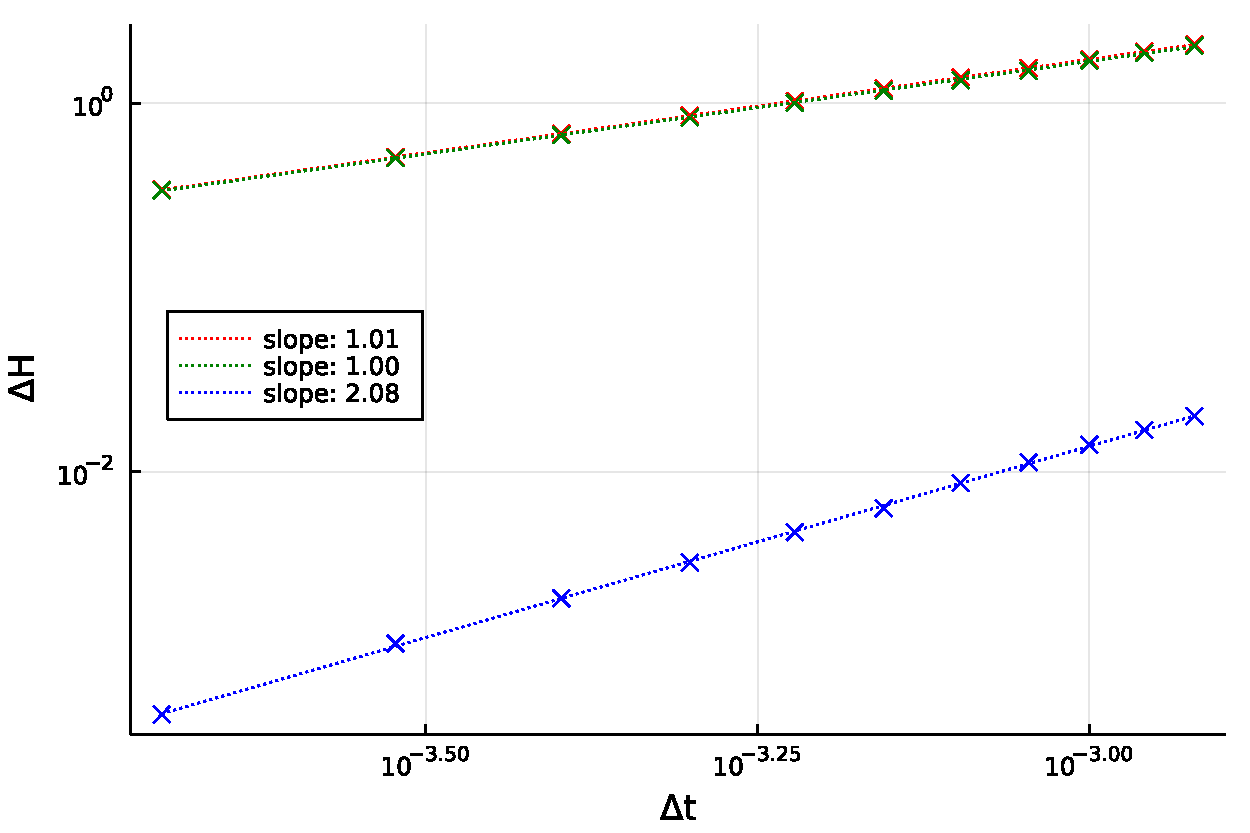
\includegraphics[width=0.7\linewidth]{figures/chapter1/hamiltonian_conservation.pdf}
          \caption{ \label{fig:hamiltonian_conservation}
            Effect of the time step on absolute variation of the Hamiltonian for the symplectic Euler (red and green) and the Verlet (blue) schemes. As expected, total variation scales as $\Delta t$ for symplectic Euler, and as $\Delta t^2$ for Verlet.
          }
        \end{center}
      \end{figure}

    \subsection{Examples of instantaneous observables}
        
    \subsection{Shortcomings of the Hamiltonian approach}

\section{Canonical averages}

\subsection{Langevin dynamics}
We consider a special case of the inertial Langevin dynamics, defined by the following stochastic differential equation (SDE), where $\gamma, \beta$ are set real constants.

\begin{equation}
    \label{Langevin}
    \left\{\begin{aligned}
        \text dq_t&=M^{-1}p_t\dt,\\
        \text dp_t&= -\nabla V(q_t)\dt \textcolor{blue}{-\gamma M^{-1}p_t\dt}+\textcolor{purple}{\sqrt{\frac{2\gamma}\beta}\text dW_t},
    \end{aligned}\right.
\end{equation}

where $(W_t)_{t\geq 0}$ is a standard $dN$-dimensional Brownian motion.

This process is a combination of a Hamiltonian evolution with an additional action on the momenta which, if isolated, defines a $dN$-dimensional Ornstein-Uhlenbeck process.\\
This additional term be interpreted physically as the combination of two effects: a \textcolor{blue}{dissipation term} which can be understood as the effect of a viscous friction force on the particles, and a \textcolor{purple}{fluctuation term}, which corresponds to the input of kinetic energy into the system as thermal agitation induced by a surrounding heat bath at temperature $1/(k_B\beta)$.\\
However, the physical meaning can be forgotten thanks to the fact that, \textit{in fine}, we only require that the canonical measure be invariant under this dynamic: as we shall shortly see, this is indeed the case.

\begin{remark}
    There are several ways to generalize this process: one is to consider more general, possibly non-separable, Hamiltonians, as in (\ref{non-separable hamiltonian}), rather than the classical Hamiltonian used above.
    The other is to allow the fluctuation-dissipation term to be parametrized by coefficients $\gamma$ and $\sigma$ depending on the state variable, and which obey a relation ensuring the invariance of $\mu$.
    Hence in full generality, we could consider the following Langevin dynamic:
    
    \begin{equation}
        \label{general Langevin}
        \left\{\begin{aligned}
            \text dq_t &=\nabla_p H(q_t,p_t)\dt,\\
            \text dp_t &= -\nabla_q H(q_t,p_t)\dt -\gamma(q_t,p_t)\nabla_pH(q_t,p_t)\dt+\sigma(q_t,p_t)\text dW_t.
        \end{aligned}\right.
    \end{equation}
\end{remark}



\subsection{Properties of the Langevin dynamics}

To investigate some of the properties of the dynamics, it is useful to introduce the notion of a generator for a process defined by a possibly inhomogeneous SDE.
\subsubsection{The generator}
We consider a general process defined by a SDE of the form:

\begin{equation}
    \label{SDE}
    \text dX_t=b(t,X_t)\text \dt + \sigma(t,X_t)\text dW_t
\end{equation}

Where $b$ is a $\R^n$-valued function, $W$ is a standard $d$-dimensional Brownian motion and $\sigma$ is a $n\times d$ matrix-valued function.\\
For $\varphi$ a smooth bounded function, Itô's lemma allows us to compute:
\begin{align*}
    d\varphi(t,X_t) &=\frac{\partial \varphi}{\partial t}(t,X_t)\text dt + \nabla^\intercal \varphi(t,X_t) \text dX_t + \frac12 \operatorname{Tr}(\nabla^{2\intercal}\varphi(t,X_t)\text d\langle X ,X\rangle _t)\\
    &=\left( \frac{\partial \varphi}{\partial t} + \nabla^{\intercal}\varphi b + \frac12 \operatorname{Tr}(\nabla^2\varphi \sigma\sigma^\intercal) \right)(t,X_t) \text dt+ (\nabla^\intercal \varphi\sigma )(t,X_t)\text dW_t,
\end{align*}

where $\nabla$, $\nabla^2$ are with respect to the spatial coordinates. In other words,


\begin{equation}
    \label{Ito}
    \varphi(t,X_t)= \varphi(0,X_0)+\int_0^t\left( \frac{\partial \varphi}{\partial t} + \nabla^\intercal\varphi b + \frac12 \operatorname{Tr}(\nabla^2\varphi\sigma\sigma^\intercal) \right)(s,X_s) \text ds + \int_0^t\nabla^\intercal \varphi\sigma(s,X_s)\text dW_s.
\end{equation}
%----invariance of $\mu$

    \begin{definition}[Generator of an Itô process]
        Let $X_t$ be a $\R^n$-valued process defined by \ref{SDE}. We define its generator at time $t$ as the operator defined by

        \begin{equation}
            \label{Generator}
            \cL_t \varphi(x)=\left(\frac{\partial \varphi}{\partial t} + \nabla^\intercal\varphi b + \frac12 \operatorname{Tr}(\nabla^2\varphi \sigma\sigma^\intercal)\right)(t,x)
        \end{equation}

    \end{definition}

    In view of (\ref{Ito}), we have, provided regularity conditions on $\sigma$ and $\varphi$,
    $$\E\left[\varphi(t,X_t)\right|X_s=x]=x+\int_s^t \E[\cL_u\varphi(X_u)] \text du$$
    so that, at least formally,
    \begin{equation}
    \label{generator formal motivation}
    \frac{\partial}{\partial t}\E[\varphi(t,X_t) | X_{s}=x]=\E[\cL_{t} \varphi(X_{t})|X_{s}=x]=\cL_{t}\E[\varphi(t,X_{t})|X_{s}=x]
    \end{equation}

    If we define a family of evolution operators $(P_{s,t})_{s\leq t}$ by the formula
    $$P_{s,t} \varphi (x)= \E[ \varphi (t,X_t) | X_s=x] $$
    (\ref{generator formal motivation}) rewrites
    $$ \frac{\partial}{\partial t} P_{s,t} \varphi (x)=P_{s,t}\cL_t\varphi(x)=\cL_t P_{s,t}\varphi(x)$$
    
    An important special case occurs when $b,\ \sigma$ and $\varphi$ do not depend on time. In this case the generator is a single operator $\cL$, defined by
    $$\cL \varphi = \nabla^\intercal \varphi b + \frac12 \operatorname{Tr}(\nabla^2 \varphi \sigma \sigma ^\intercal)$$ 
    The evolution operators $P_t \defeq P_{0,t}$ ($ = P_{s,s+t}\ \forall s$ by stationarity) form a semi-group, and act on the space of smooth functions as
    $$ P_t \varphi(x)= \E[\varphi(X_t)| X_0=x]$$
    The formal derivative is given by
    $$ \frac{\partial}{\partial t}P_t=P_t\cL=\cL P_t$$
    
    As in (\ref{evolution operator exponential notation}), we may write, by analogy with the finite-dimensional setting,
    $e^{t\cL}\defeq P_t$


    \subsubsection{Invariance of the canonical measure}

    The Langevin dynamics (\ref{Langevin}), when written under the form (\ref{SDE}), corresponds to the case 

    $$ b(q,p)= \begin{pmatrix} M^{-1}p \\ -
    \nabla V(q)-\gamma M^{-1}p\end{pmatrix},\ \sigma(q,p)= \sqrt{\frac{2\gamma}\beta}\begin{pmatrix} 0_{dN} &  0_{dN} \\  0_{dN} & \text{I}_{dN} \end{pmatrix}$$
    Hence, applying \ref{Generator}, we obtain the generator for the dynamics
    $$ \cL=  \cL_q + \cL_p $$
    where
    $$ \cL_q \varphi= \nabla^\intercal_q\varphi M^{-1}p$$
    $$ \cL_p\varphi =-\nabla^\intercal_{p}\varphi (\nabla V(q)+\gamma M^{-1}p) +\frac{\gamma}{\beta}\Delta_p $$
    which we may rewrite, recognizing the generator for the Hamiltonian dynamics \ref{Hamiltonian generator}
    $$ \cL=\cL_{H}+\gamma \cL_{\text{ou}}$$
    where $\cL_{\text{ou}}\varphi =-M^{-1}\nabla^\intercal_p\varphi p + \frac1{\beta}\Delta_p\varphi$

\section{Numerical schemes for the Langevin dynamics}
text
    \subsubsection{Splitting methods}
    text
    \subsubsection{Implementation}
    text
    \begin{figure}[htbp]
        \begin{center}
            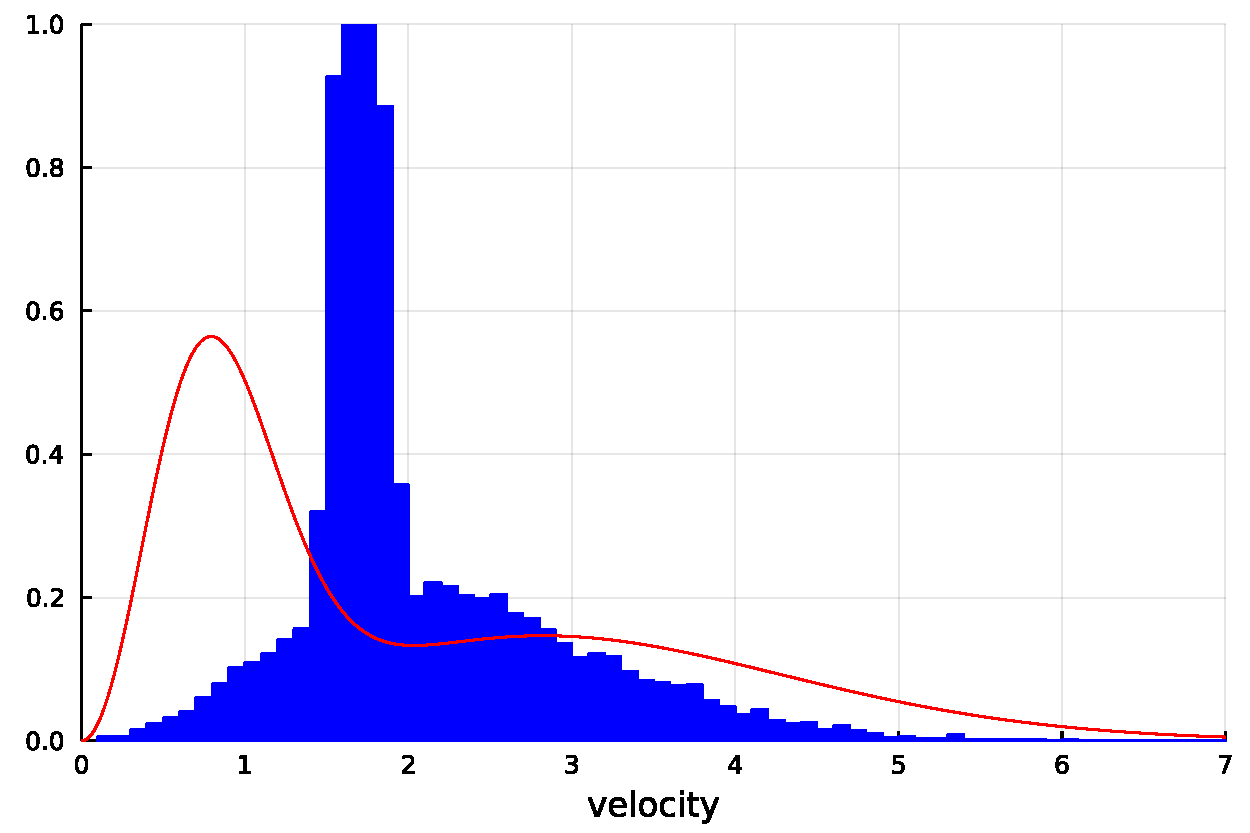
\includegraphics[width=0.49\linewidth]{figures/chapter1/velocities_20.pdf}
            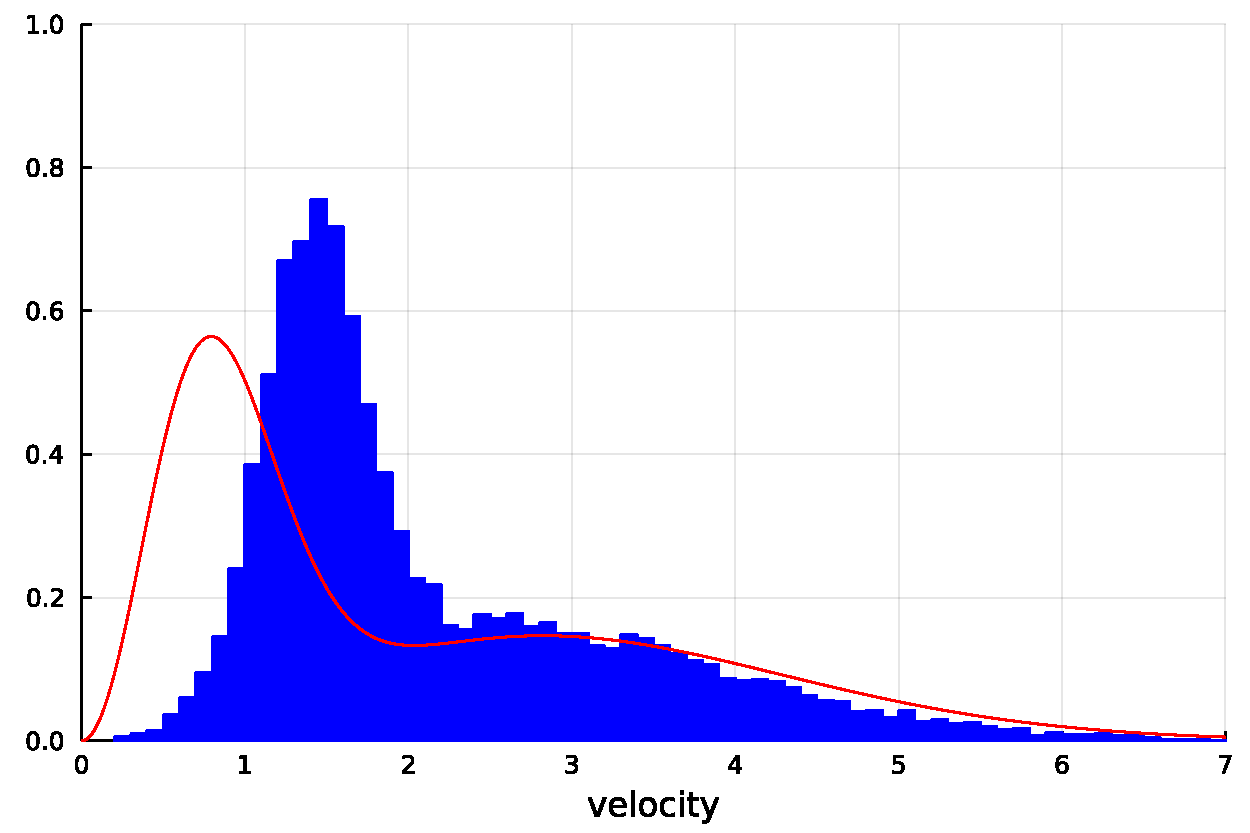
\includegraphics[width=0.49\linewidth]{figures/chapter1/velocities_200.pdf}
            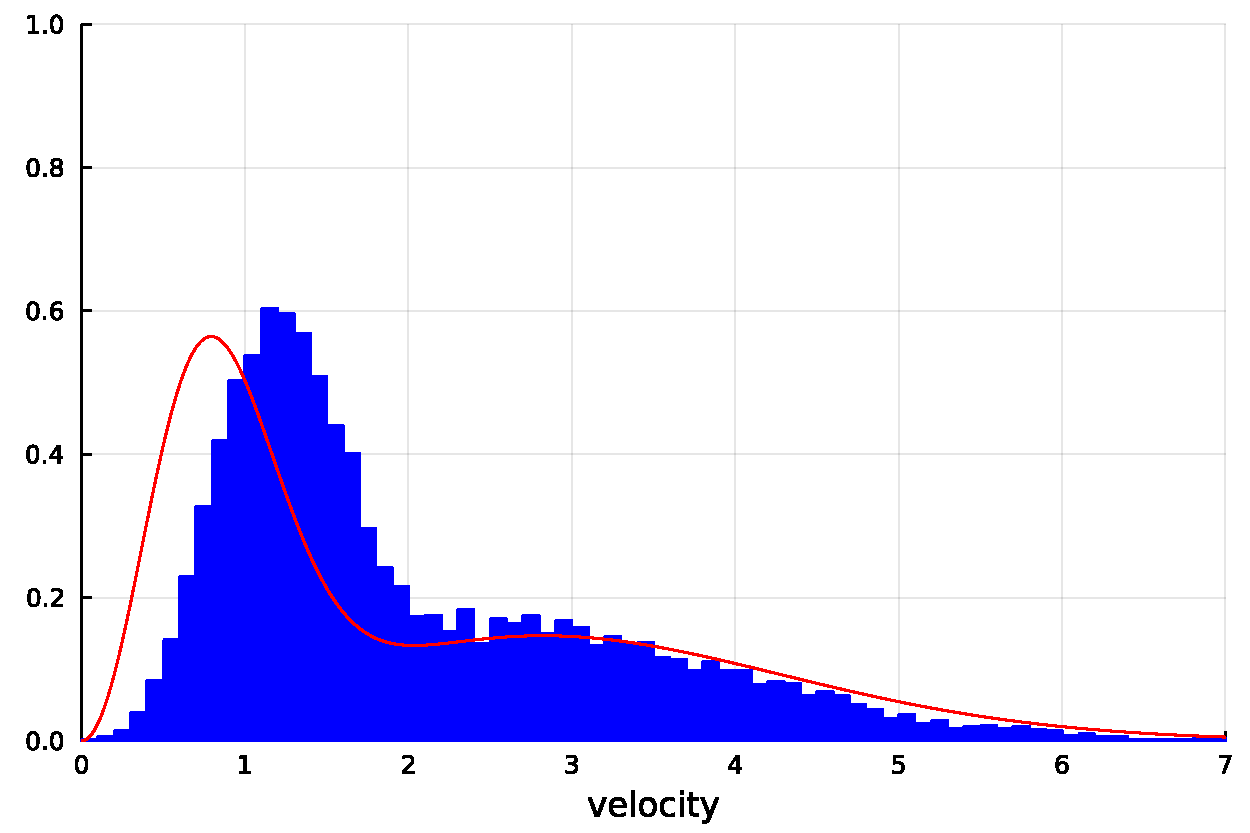
\includegraphics[width=0.49\linewidth]{figures/chapter1/velocities_400.pdf}
            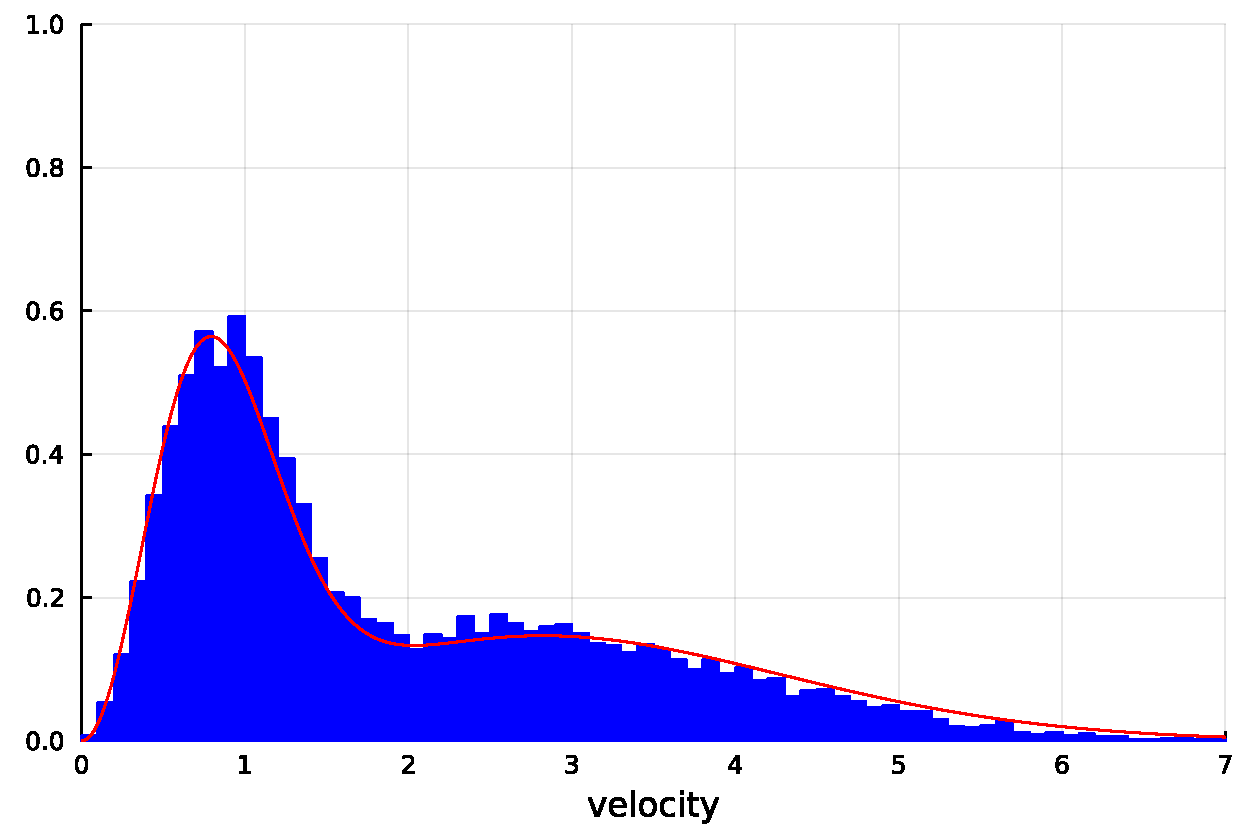
\includegraphics[width=0.49\linewidth]{figures/chapter1/velocities_1000.pdf}
          \caption{ \label{fig:velocity_histograms}
            Convergence of the velocity distribution to a mixture of Maxwell-Boltzmann distributions (plotted in red) for a mixture of two ideal gases with different atomic masses, starting from a Dirac distribution $\delta_{\sqrt 3}^{\otimes N}$. Snapshots of the empirical distribution are shown after 20,\ 200,\ 400 and 1000 steps ($\Delta t=5\times 10^{-3} \tau ^*, T=T^*$)          }
        \end{center}
      \end{figure}


\subsection{Error analysis for splitting schemes}
\begin{figure}[htbp]
    \begin{center}
      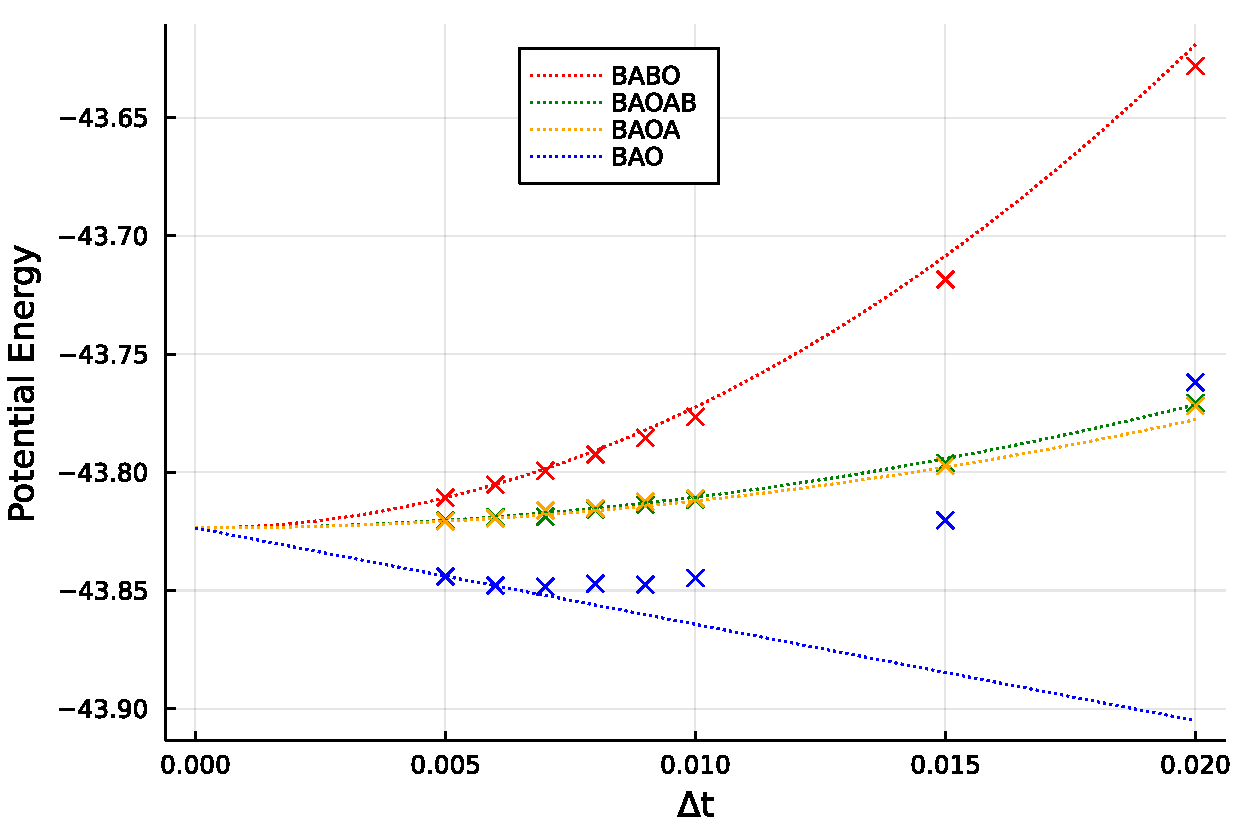
\includegraphics[width=0.49\linewidth]{figures/chapter1/potential_energy_bias.pdf}
      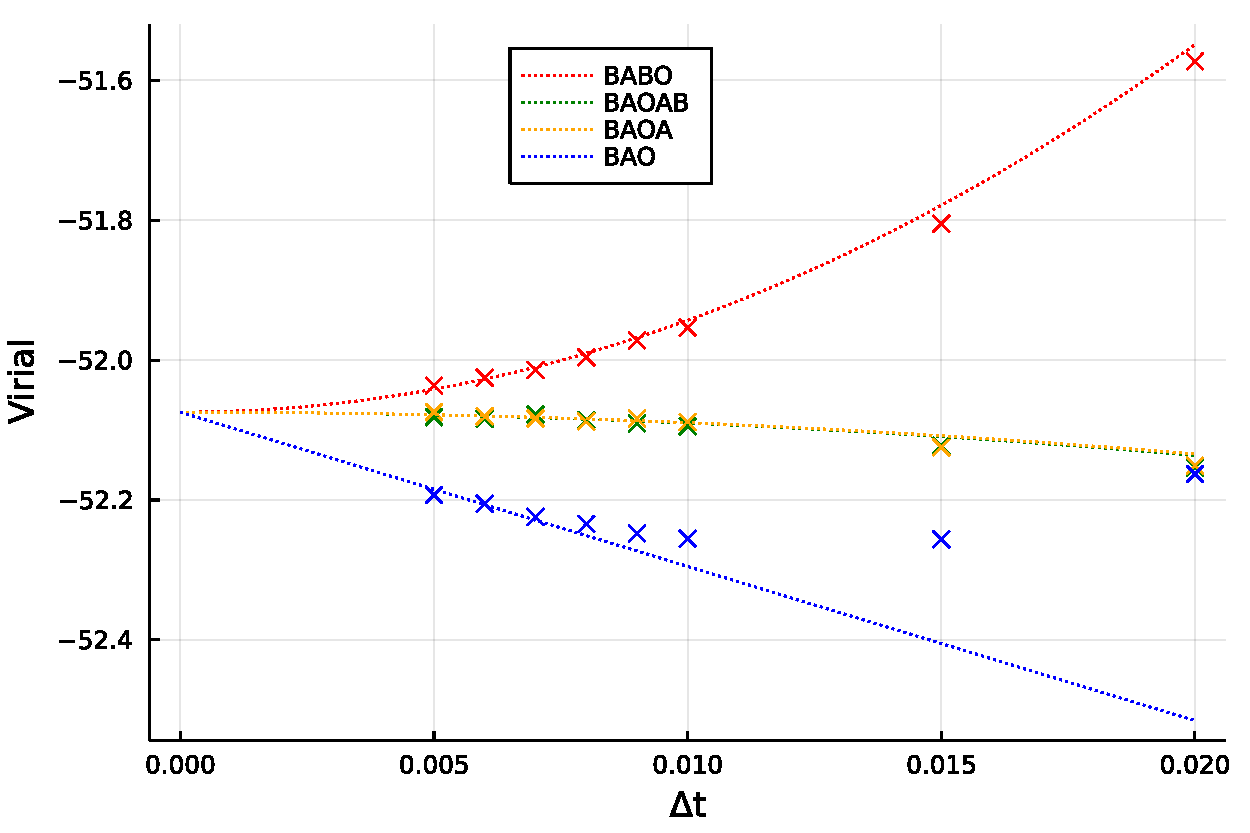
\includegraphics[width=0.49\linewidth]{figures/chapter1/virial_bias.pdf}
      \caption{ \label{fig:configurational_bias}
        Effect of the time step on average potential energy and virial for a Lennard-Jones system of 27 particles.
      }
    \end{center}
  \end{figure}

  \begin{figure}[htbp]
    \begin{center}
      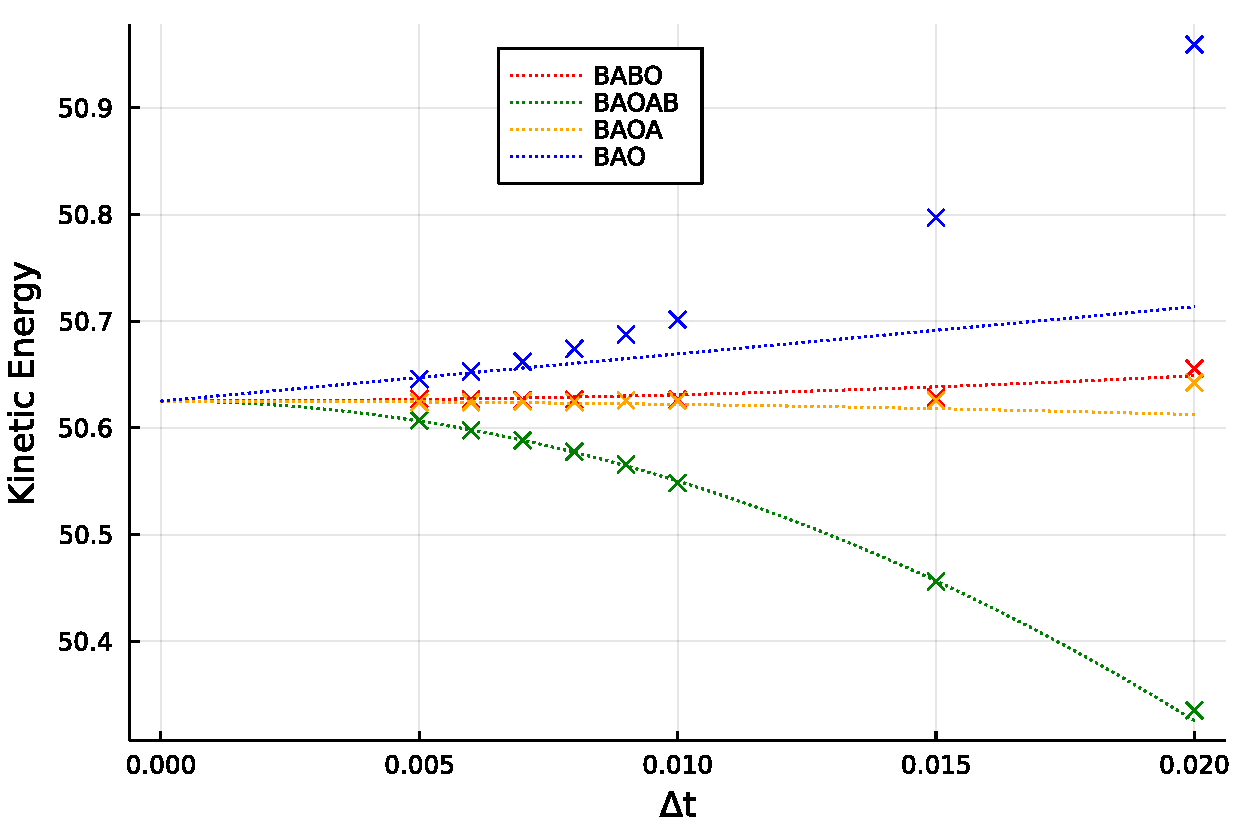
\includegraphics[width=0.7\linewidth]{figures/chapter1/kinetic_energy_bias.pdf}
      \caption{ \label{fig:kinetic_energy_bias}
        Effect of the time step on average kinetic energy for a Lennard-Jones system of 27 particles.
      }
    \end{center}
  \end{figure}

To explain the overlap of bias between the BAOAB and the BAOA schemes observed for the potential energy and virial on Figure \ref{fig:configurational bias}, we use the following result, which is a variation on the TU lemma.
\begin{lemma}\label{TU_like_lemma}
    Let $P_{\Delta t}, Q_{\Delta t}$ be bounded operators on $B^\infty(\mathcal E)$.
    Assume that, for any $n\geq 1$,
    $$ A P_{\Delta t}^n = Q_{\Delta t}^n B,$$
    where $A$ and $B$ are bounded operators on $B^\infty (\mathcal E)$, such that $A\1=\1$, and that the following ergodic condition holds: for any $\varphi \in B^\infty(\mathcal E)$, and almost all $(q,p) \in \mathcal E$,

    $$ \underset{n\to\infty}\lim P_{\Delta t}^n\varphi (q,p) = \int_{\mathcal E} \varphi(q,p)\mu_{\Delta t,P}(\text d q,\text d p) $$
    $$ \underset{n\to\infty}\lim Q_{\Delta t}^n\varphi (q,p) = \int_{\mathcal E} \varphi(q,p)\mu_{\Delta t,Q}(\text d q,\text d p).$$

    Then  we can relate $\mu_{\Delta t,P}$ and $\mu_{\Delta t,Q}$ via the following relation:

    \begin{equation}
        \label{TU_like_lemma_ccl}
    \int_{\mathcal E} \varphi(q,p) \mu_{\Delta t,P}(\text d q,\text d p)=\int_{\mathcal E} B\varphi(q,p) \mu_{\Delta t,Q}(\text d q,\text d p)
    \end{equation}
    \begin{proof}
        Fix an initial probability measure $\rho$ on $\mathcal E$, absolutely continuous with respect to the Lebesgue measure. Then we may write, using dominated convergence to pass to the limit:

        \begin{align*}
            &\int_{\mathcal E}AP_{\Delta t}^n \varphi(q,p)\rho(\text d q,\text d p)\\
            &=\int_{\mathcal E}P_{\Delta t}^n \varphi(q,p)A^{\dagger}\rho(\text d q,\text d p)\\
            &\underset{n\to\infty}{\longrightarrow}\int_{\mathcal E} \left (\int_{\mathcal E}\varphi(q,p)\mu_{\Delta t,P}(\text d q,\text d p)\right) A^\dagger \rho(\text d \tilde q,\text d \tilde p)\\
            &=\int_{\mathcal E}\varphi(q,p)\mu_{\Delta t,P}(\text d q,\text d p)\int_{\mathcal E}A\1 \text d \rho\\
            &=\int_{\mathcal E}\varphi(q,p)\mu_{\Delta t,P}(\text d q,\text d p)
        \end{align*}
        Furthermore, applying the ergodic condition to the bounded function $B\varphi$ gives

        $$ \int_{\mathcal E} Q_{\Delta t}^n (B\varphi)(q,p) \rho(\text d q,\text d p) \text d q \text d p \underset{n\to\infty}{\longrightarrow}\int_{\mathcal E} \left (\int_{\mathcal E}B\varphi(q,p)\mu_{\Delta t,Q}(\text d q,\text d p)\right)\rho(\text d \tilde q,\text d \tilde p)=\int_{\mathcal E}B\varphi(q,p)\mu_{\Delta t,Q}(\text d q,\text d p).$$

        Since $AP_{\Delta t}^n=Q_{\Delta t}^n B$, identifying the two limits yields (\ref{TU_like_lemma_ccl})
    \end{proof}
\end{lemma}

\begin{corollary}
Let $ \pi_{\Delta t}$ and $\pi_{\Delta t}'$ be the invariant measures for the Markov transition operators defined respectively by the BAOA and BAOAB schemes for a fixed timestep $\Delta t$. Then the corresponding marginal distributions on $\mathcal D$ are equal.

\begin{proof}
    We denote by $P_{\Delta t}$ the transition operator for the BAOA scheme, and similarly $Q_{\Delta t}$ for the BAOAB scheme. It is straightforward to check that 
    $$ e^{\frac{\Delta t}2 B}P_{\Delta t}^n=Q_{\Delta t}^n e^{\frac{\Delta t}2 B}.$$

    Assuming the ergodic condition of Lemma \ref{TU_like_lemma} (TODO check doeblin condition), we can apply the result to get, for any bounded measurable observable $\varphi$,

    $$ \int_{\mathcal E} \varphi(q,p)\pi_{\Delta t}(\text d q,\text d p)=\int_{\mathcal E} e^{\frac{\Delta t}2 B}\varphi(q,p)\pi'_{\Delta t}(\text d q,\text d p)$$

    Now if $\varphi (q,p)= \varphi (q,0) \defeq \varphi(q)$ for all $p$, then $e^{\frac{\Delta t}2 B}\varphi=\varphi$, which yields the desired conclusion:

    $$\forall \varphi \in B^\infty(\mathcal D),\ \int_{\mathcal E} \varphi(q)\pi_{\Delta t}(\text d q,\text d p)=\int_{\mathcal E}\varphi(q)\pi'_{\Delta t}(\text d q,\text d p).$$
\end{proof}

\end{corollary}

\subsection{Application: the equation of state of Argon}
text
\begin{figure}[htbp]
    \begin{center}
      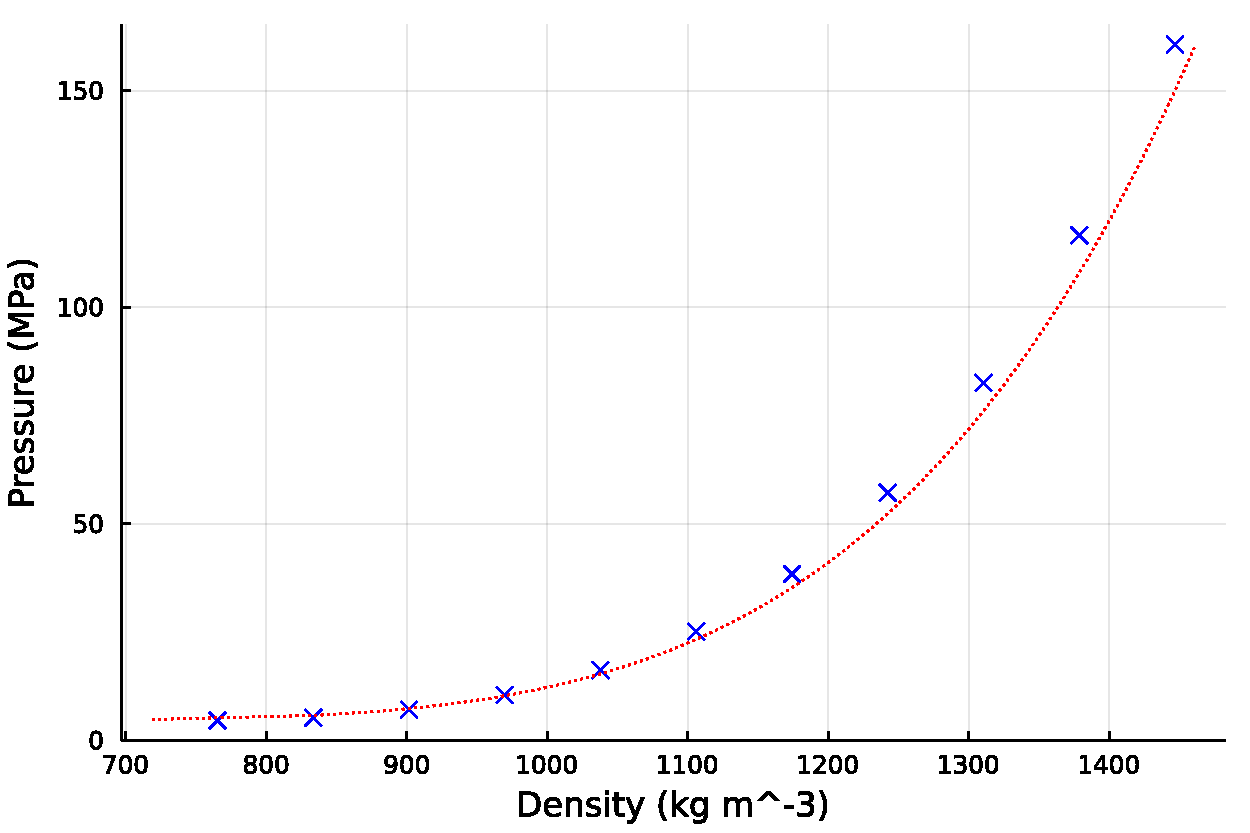
\includegraphics[width=0.49\linewidth]{figures/chapter1/argon_nvt_150K.pdf}
      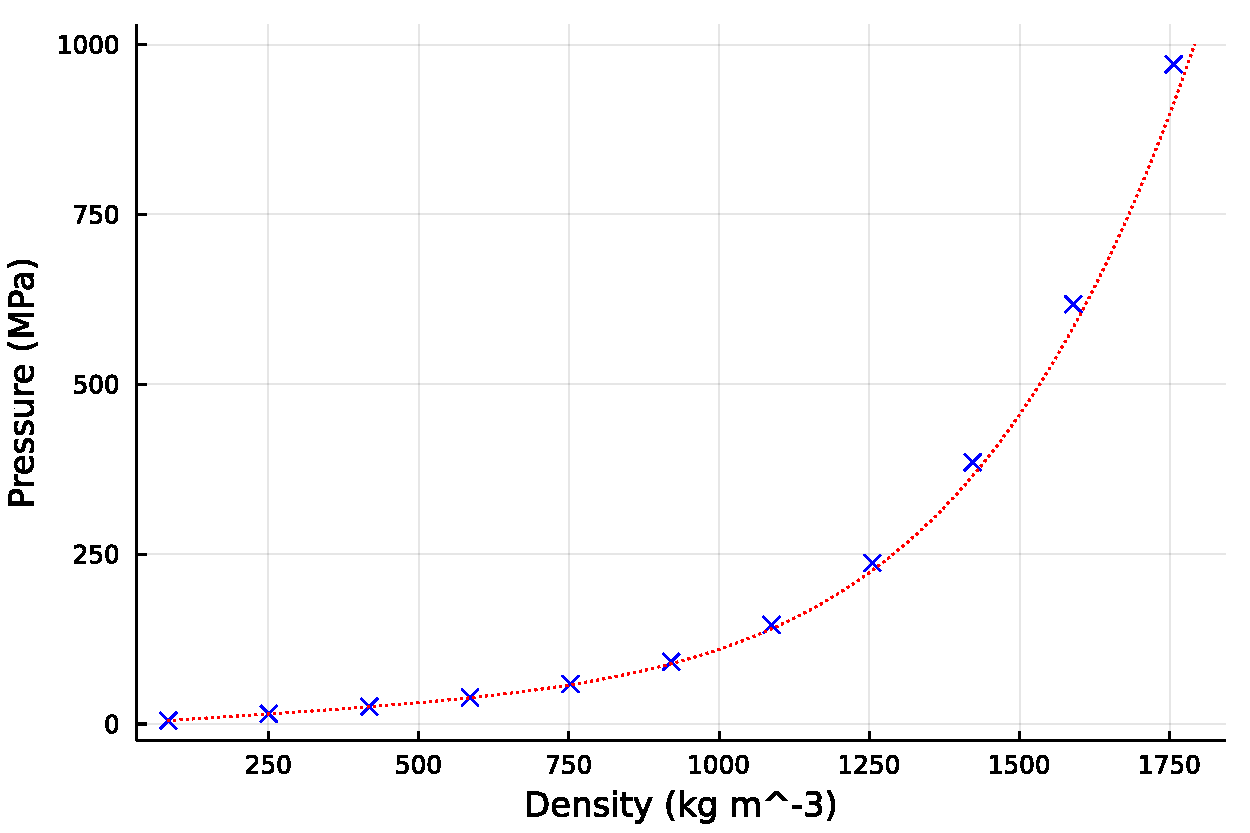
\includegraphics[width=0.49\linewidth]{figures/chapter1/argon_nvt_300K.pdf}
      \caption{ \label{fig:eos_argon}
        Simulated equations of state of Argon at 150 K (liquid phase, left) and 300 K (supercritical phase, right). Experimental reference curves are plotted in red, simulated data points are scattered in blue.
      }
    \end{center}
  \end{figure}
\subsection{The Metropolis method}